\section{Resultados}

O tipo de plantação base usado para esse trabalho foi a Cana-de-açúcar, mas outros tipos de plantio foram testados e se obteve o resultado desejado. Por esse motivo os resultados que serão apresentados, tem como plantio base a Cana-de-açúcar.

Segue abaixo algumas das regras de produção utilizadas: 

\begin{figure}[h!]
\centering
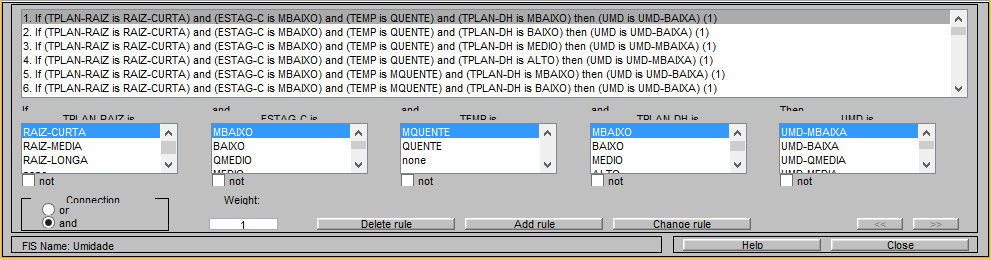
\includegraphics[width=1\linewidth]{Resultados/Imagens/regras}
\caption{Regras de produção}
\label{fig:Regras}
\end{figure}

Como exemplo começaremos atribuindo os seguintes valores para as variáveis de entrada:

TPLAN-RAIZ: RAIZ-MEDIA

ESTAG-C: BAIXO

TEMP: QUENTE

TPLAN-DH: BAIXO

Obtemos o seguinte resultado:

\begin{figure}[h!]
\centering
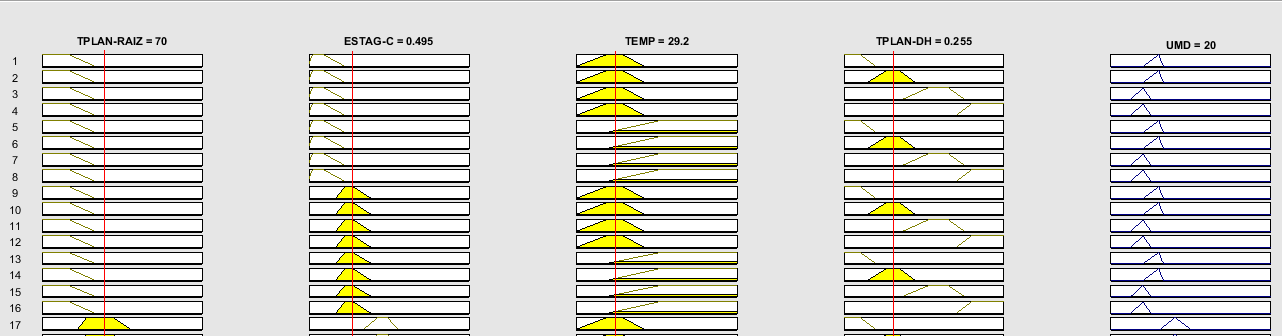
\includegraphics[width=1\linewidth]{Resultados/Imagens/resultado1}
\caption{Resultado 1}
\label{fig:resultado1}
\end{figure}

Nessas condições a variável de saída UMD é igual a 20. Se alterarmos as variáveis de entrada da seguinte forma:  

TPLAN-RAIZ: RAIZ-MEDIA

ESTAG-C: ALTO

TEMP: MQUENTE

TPLAN-DH: BAIXO

Obtemos o seguinte resultado:

\begin{figure}[h!]
\centering
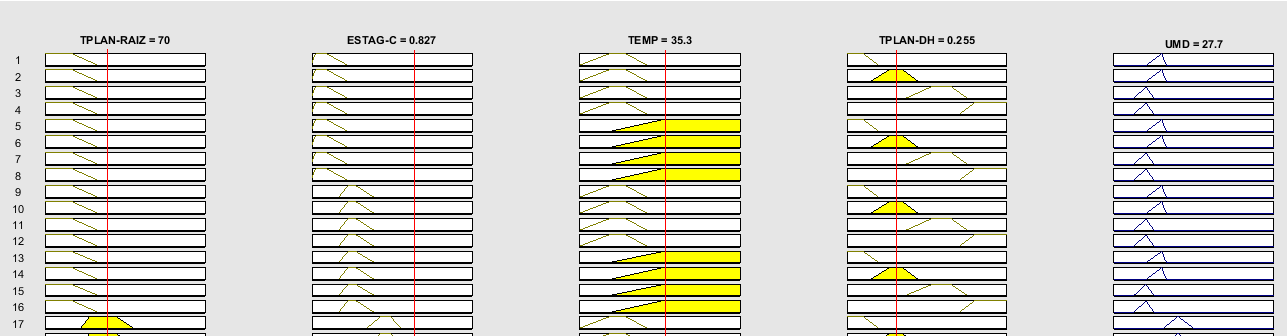
\includegraphics[width=1\linewidth]{Resultados/Imagens/resultado2}
\caption{Resultado 2}
\label{fig:resultado2}
\end{figure}

Como esperado com o estágio de crescimento da planta alterado para alto (floração), o qual requer um maior consumo hídrico, e a temperatura alterada para muito quente, a umidade ideal para o solo aumenta para 27,7. Com base nesses resultados concluímos que o sistema fuzzy implementado correspondeu as expectativas do projeto. 
